\documentclass[11pt]{article}
\usepackage{cite}
\usepackage{url}
\usepackage{graphicx}
\usepackage{wrapfig}
\usepackage{setspace}

\usepackage[margin=0.75in]{geometry}

\title{Efficient Discovery of Regular Patterns in Iregular Programs and Its Use in Compiler Prefetching}

\author{Patryk Mastela, Jason Varbedian, Matt Viscomi \\
  \small {\texttt {\{pmastela,jpvarbed,mviscomi\}@umich.edu}}}

  \date{\today}

  \doublespacing
  \begin{document}
  \maketitle
  \begin{abstract}
    Large latency delays exist when transferring requests from main memory to the cache during load instructions. If the data is already in the cache, the latency to retrieve that information is much lower, as main memory does not have to be accessed. Therefore, before load instruction executes, if the data being requested is already in the cache, the application’s overall performance can be increased. Prefetching is an approach that can be taken to attain this performance boost. The particular problem we explore is finding regular stride patterns in irregular programs. Since loads typically occur in patterns, we were able to analyze a program’s set of loads to look for those patterns. There are three types of patterns that typically occur during the profiling step: strong single stride loads, phased multi-stride loads, and weak single stride loads. We will explain the profiling of stride values and analyze the results which illustrate overall positive performance gains in the experiments from inserted prefetch instructions.
  \end{abstract}
  \section{Introduction}
  Irregular programs contain many irregular data references, e.g., pointer-chasing code that manipulates dynamic data structures. Because of this irregularity of data references it is hard for both the compiler and hardware to anticipate the future address of a memory location. Others, including Collins et al.~\cite{collins01}, Stoutchinin et al.~\cite{stoutchinin01}, and Wu et al.~\cite{WuEtAl2002}, have noticed that important loads in benchmark suite programs, e.g., in CPU2000, have near-constant strides. Many other benchmarks in CPU2000 also exhibit near-constant strides. With the consistency of near-constant stride occurrence throughout the benchmark suite there is an opportunity for an ultimate run time performance gain at the cost of an upfront payment at compile time. 
  \\\\The process of exploiting regular stride patterns in irregular programs is called stride profiling. A stride value is the difference between two consecutive load addresses. It consists of identifying candidate loads~\cite{WuEtAl2002}. In order for a load to be classified as a candidate it must satisfy three conditions:
  \begin{itemize}
    \item Execute more than 2000 times
    \item Must occur inside of a loop which is executed at least 128 times
    \item The memory location is not loop invariant.
  \end{itemize}
  The reason for this set of properties is that profiling can possibly take an extended period of time. To reduce this overhead we chose to only profile loads that are executed within loops with high execution counts; this discriminating approach to selecting loads is noted by Wu et al.~\cite{WuEtAl2002} leads to a significant reduction in the profiling overhead. Other optimizations discussed later in the paper are also applied that trade a small amount of run time performance for a smaller profiling overhead.
  \\\\There are several steps before arriving at the end goal of prefetching instructions. First the loads must qualify for profiling, later they are grouped into different groups depending on stride values~\cite{Wu2002} and stride differences~\cite{Wu2002}. Depending on which of the load groups it falls into, i.e., strong single stride, phased multi-stride, or weak single stride load, a different set of instructions are instrumented to maximize cache hits, while minimizing unnecessary memory accesses if the load is not a popular one.
  \\\\The rest of the paper is organized as follows. Section 2 overviews [TODO]. Section 3 provides [TODO]. Section X concludes the paper.
  %\subsection{this is an intro subsection}
  \section{Profiling}
  There are two main phases to our project, run-time load profiling and prefetch instruction insertion. The two must be separated because the profiling phase gathers run-time information about the source code with a transformative pass. These transformation changes slow the source code so we must do our insertions in a different pass.
  \\\\Profiling overhead for each load is large so we only choose loads with promising profiles. Using an edge frequency and loop info pass we select loads only with certain criteria. The loads must be in loop loads, have a \textit{trip count} (the number of times a loop executes) of at least 128, and have addresses that aren’t loop invariant. The reason for this is that in-loop loads have patterns, and have to execute enough times that we can do calculations until the prefetch completes. Additionally, loads must have loop invariant addresses so that the address changes within the loop. We decide if a load is loop invariant by looking at the load’s pointer operand. If that instruction is loop invariant so is the load instruction.
  \\
  \begin{figure}[h]
    \centering
    \begin{minipage} [b] {7.5cm}
      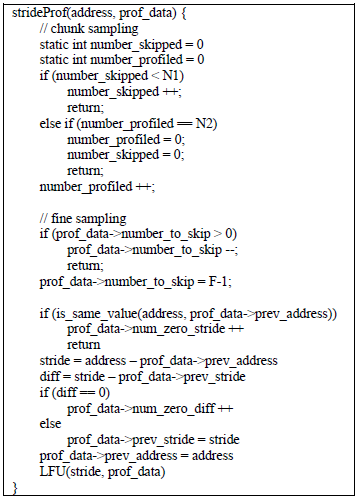
\includegraphics[scale=0.6]{./img/fig9}
      \caption{Pointer-chasing code with stride patterns\label{stride patterns}}
    \end{minipage}
    \begin{minipage} [b] {7.5cm}
      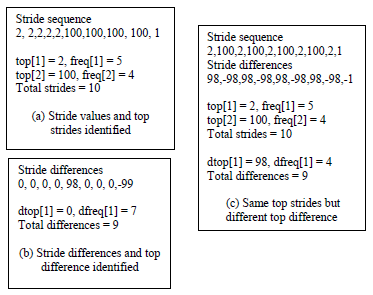
\includegraphics[scale=0.6]{./img/fig4}
      \caption{Stride value and stride difference profile example\label{fig4}}
    \end{minipage}
  \end{figure}
  \\For each load that we select to profile, we insert a sampling control flow to a class that collects the top four stride values, their frequencies and the number of zero differences in the stride pattern, and the number of times the stride is zero. This information is then output to a file for the next phase of the project to read in as input. The control flow is necessary to sample a certain amount of loads. We sample about 30 loads, skip a certain percentage, sample an additional 30, and repeat that procedure. See Figure~\ref{stride patterns} for a high level code of how the profiler is implemented. N1 in the code is the number of addresses to skip from profiling, and N2 is the number of times that the load is profiled. During the profiling step we instrument the code on the profiled loads to execute the code in assembly. This is one difference from the paper, instead of doing the counting and checks in a hook, we do modify the assembly directly. We found this to increase the time of our performance.
  \\\\The actual profiling was done in a hook call, Stride\_AddAddress, for each address we profiled. Each load had a separate class instance assigned to it in order to keep track of the number of strides, number of \textit{zero difference strides} (difference between two consecutive stride values), the number of \textit{zero strides} (difference of two consecutive addresses is zero), the \textit{dominant stride} (the stride value that occurs the most frequently), and the top four
  frequent stride frequencies. See Figure~\ref{fig4} for an example.
  These values are then written to a file during the pass which is read during our prefetch instruction insertion pass to determine the prefetch value, and whether the load is actually worth prefetching.
  \begin{figure}[h]
    \centering
    \begin{minipage} [b] {8cm}
      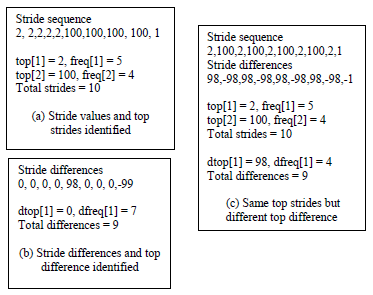
\includegraphics[scale=0.6]{./img/fig4}
      \caption{Stride value and stride difference profile example\label{fig4}}
    \end{minipage}
    \begin{minipage} [b] {7cm}
      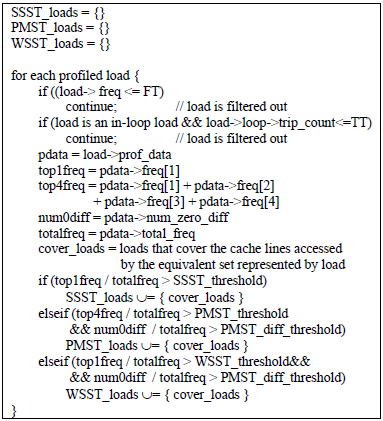
\includegraphics[scale=0.6]{./img/fig5}
      \caption{Identify prefetched loads during profile feedback\label{fig5}}
    \end{minipage}
  \end{figure}


  \section{Prefetch Insertion}
  In the prefetch insertion phase of our project, we read in the results file produced by the profiling pass and decide where to insert prefetch instructions. It uses the information gathered from the profiling pass with edge frequency pass to identify loads that will benefit from prefetching. Loads that may benefit from prefetching follow certain stride patterns~\cite{Wu2002}. If a load’s stride pattern is of one of the following, then we prefetch:
  \begin{itemize}
    \item Strong single stride (SSST) load:  a load with at least one non-zero  stride that occurs at least 70\% of the time, called the SSST\_threshold
    \item Phased multi-stride (PMST) load: a load with strides that occur in groups at least 60\% of the time, called the PMST\_threshold, with stride differences being zero at least 40\% of the time, called the PMST\_diff\_threshold
    \item Weak single stride (WSST) load: a load with only one non-zero stride at occurs at least 25\% of the time, called the WSST\_threshold, and stride differences being zero at least 10\% of the time, called the WSST\_diff\_threshold (e.g. a load has a stride of 64 25\% of the time and stride zero differences 10\% of the time)
  \end{itemize}
  We place loads in their corresponding sets if they match the criteria using the following algorithm. 
  \\\\The FT is the frequency threshold that a load must meet which we define to be 2000 from experimentation. Similarly, the TT is the trip count threshold which we set as 128.
  \\\\The next part of prefetch phase of our project is inserting the prefetch instructions and those that prepare the prefetch. Let S be the most frequently executed stride and P be the address of the load about to be executed. The K value, prefetch distance, is used as an estimation for how far ahead we should prefetch. It is determined by compile time analysis. We calculate K by estimating the number of cycles a load miss induces as 200 and how many instructions are executed in the loop. We estimate each instruction in the loop to be approximately one cycle.
  \\\\For SSST loads, we calculate at compile time \(K*S\) and insert an addition of \(K*S+P\) and finally \texttt{llvm.prefetch(P+K*S)}. For PMST loads, we store the address of the load in a scratch register, a subtraction instruction \texttt{sub(P-scratch)} and finally \texttt{prefetch(P+K*sub\_result)}. For WSST loads, we insert the same scratch and subtraction instructions, but add in a new block that does the prefetch instruction. We branch to this block when the result of the subtraction equals the dominant stride of the load.
  \section{Experiments}
  The development and experimenting was done on \textit{andrew}, a quad-core Xeon 5130-powered server clocked at 2GHz with 4MB of L2 cache per core and a cache block size of 64 bytes. Because this was a shared server amongst the rest of the students in the class sometimes the load would get heavy while our tests were running so we’d like to note that while we think our regular stride prefetching adds a performance boost many of the result anomalies could be attributes to spikes in the server’s load. 
  \\\\K is the constant that determines the prefetch distance. This constant determines which address should be fetched. A higher value would mean fetching data from memory that will be used many iterations later than if a smaller K value was used. A precise approximation of K can significantly boost performance because a value that is wrongfully large will mean that the data might get kicked out of cache before it has been used, and a K too low could prove useless if the data is already in the cache.
  \\\\We carried out experiments to examine this constant for two reasons: it is mentioned in Wu~\cite{Wu200} and, for as important as we recognize this constant to be, its evaluation is not explored in thorough detail as it should be; we wanted to find out how well-tuned our selection of K was. 
  \\\\The two ways to determine K: one relies more heavily on information about the cache, while the other doesn’t really take the cache properties into consideration and solely works off of trip count. 
  \subsection{Cache Property Approach}
  \label{sec:cache_prop_approach}
  The total size of the data area that is being referenced by a stride prefetch is trip\_count * stride. It takes \textit{L} cycles for miss latency if this referenced data area is greater than the cache level. The other important variable in this approach is the number of instructions between another hit to the same address; we will call this \textit{B} cycles which is the number of cycles that the loop body takes without taking the miss latency of prefetched loads into account. With these
  two constants in mind K can be computed as:
  \begin{equation}
    min(\lceil L/B \rceil, C) 
    \label{eqn:cache_prop_approach}
  \end{equation}
  C is the maximum prefetch distance which is our case was set to 8~\cite{Wu2002}. 
  \subsection{Trip Count Approach}
  This approach is simpler than the first approach. It solely involves the trip count and the the trip count threshold, \textit{TT}. K is therefore calculated as:
  \begin{equation}
    min(\rceil trip\_count, TT\rceil, C)
    \label{eqn:trip_count_approach}
  \end{equation}
  The threshold we selected was 128 as suggested in~\cite{Wu2002}. 

  \subsection{Our Approach}
  \label{sec:our_approach}
  Finally, our approach was a modification of the first approach. We assumed that the memory latency is 200; this value was calculating assuming that a main memory reference is about 100ns and the processor speed was 2GHz which means \(\frac{2*2^{30}}{10^9*100} = 214\). We also calculated the average number of cycles, \textit{AC}, (assuming each instruction is 1 cycle each) before the same load that would be prefetched was accessed again. We found this to be a rather good compromise since the task of getting a perfect count of cycles was non-trivial.
  \\\\We created many example applications in the C programming language that would simulate very poor cache performance. For example, we created a matrix multiplication application that would give us poor cache results. This was implemented by creating a two-dimensional array with a dimension size larger than the cache line size. Thus, by incrementing the first dimension by more than the cache line size, we are able to produce poor cache performance since a new cache line will have to be
  brought in each time.

  \section{Results}
  We tested on various tests including ones from the SPECINT2000 benchmark and also some of our own hand-crafted test cases. The results varied in terms of a performance boost, but the majority of tests proved our hypothesis that our implementation would result in speed up. 
  \begin{figure}[h]
    \begin{minipage} [t] {8.6cm}
      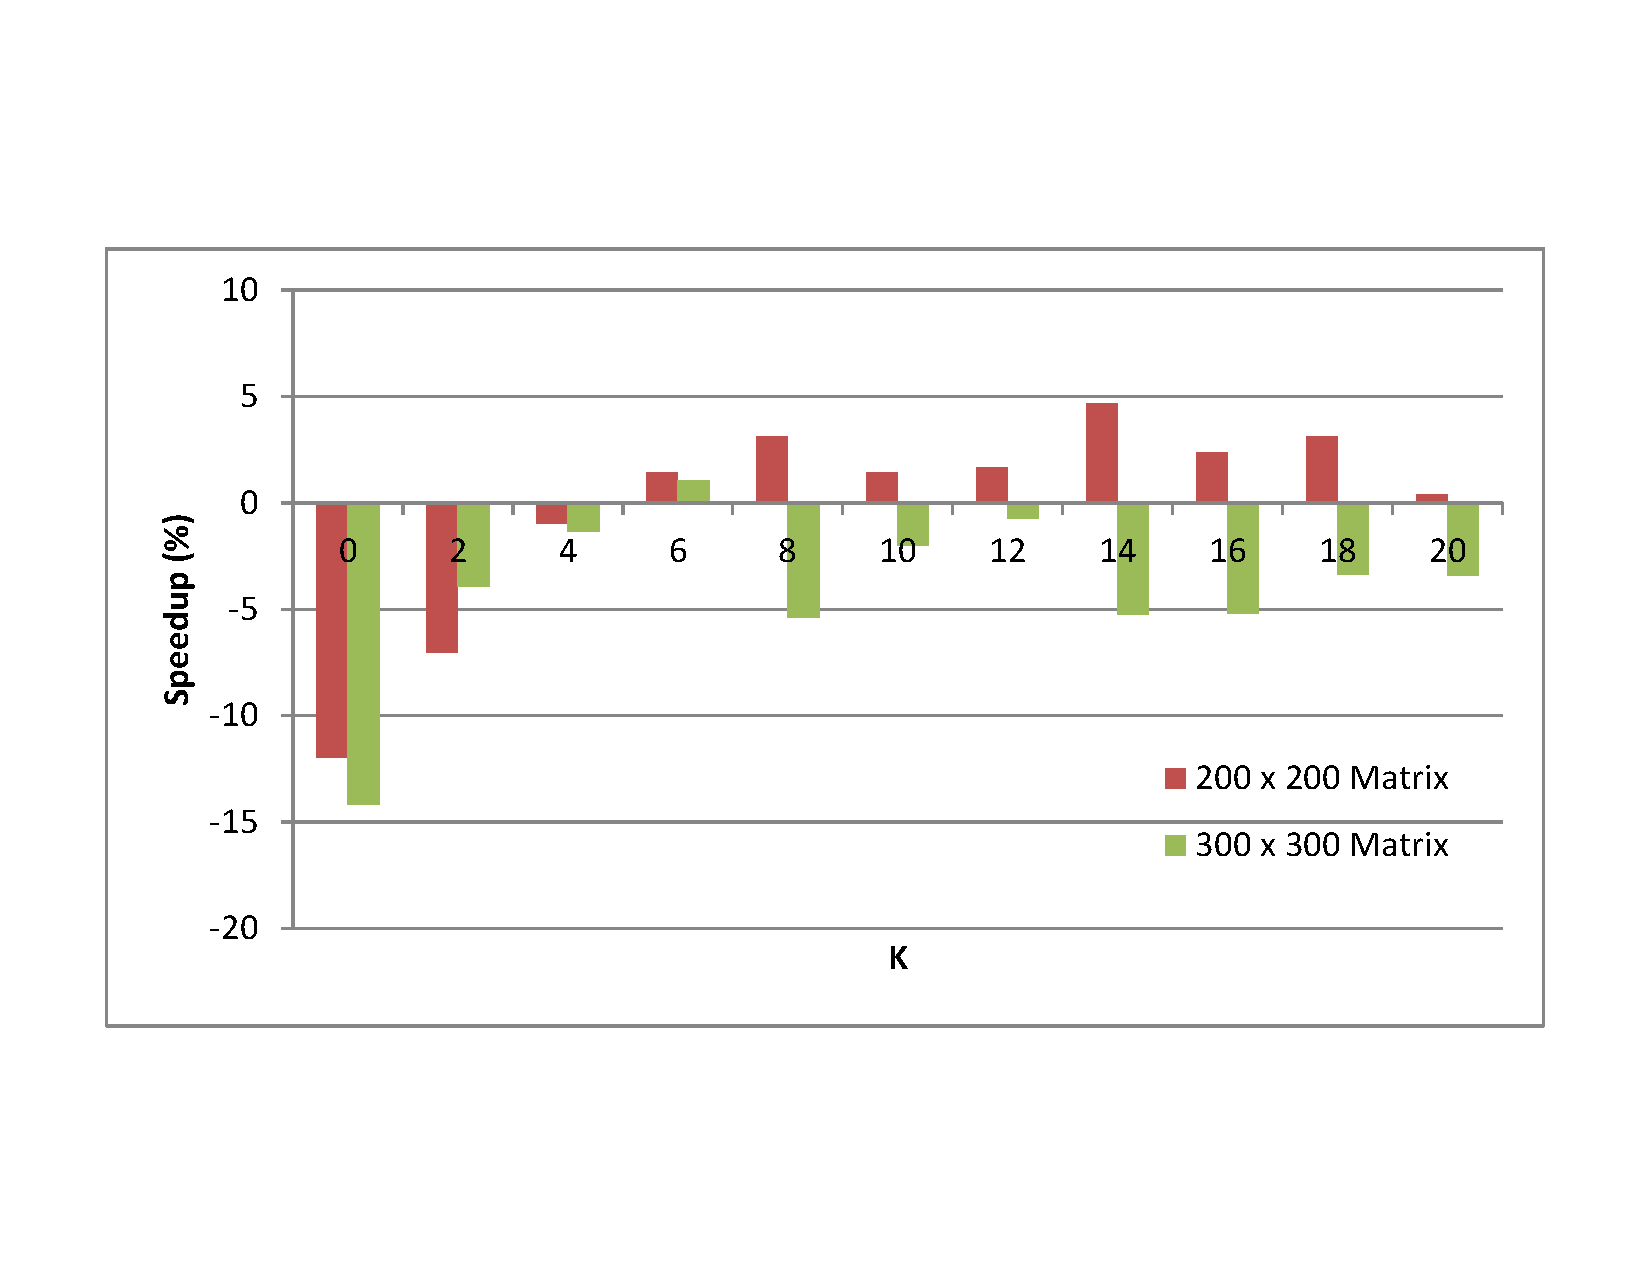
\includegraphics[scale=0.35]{./results/test_matrix1}
      \caption{Simple matrix multiplication results with varying K\label{test_matrix1}}
    \end{minipage}
    \begin{minipage} [t] {8.5cm}
      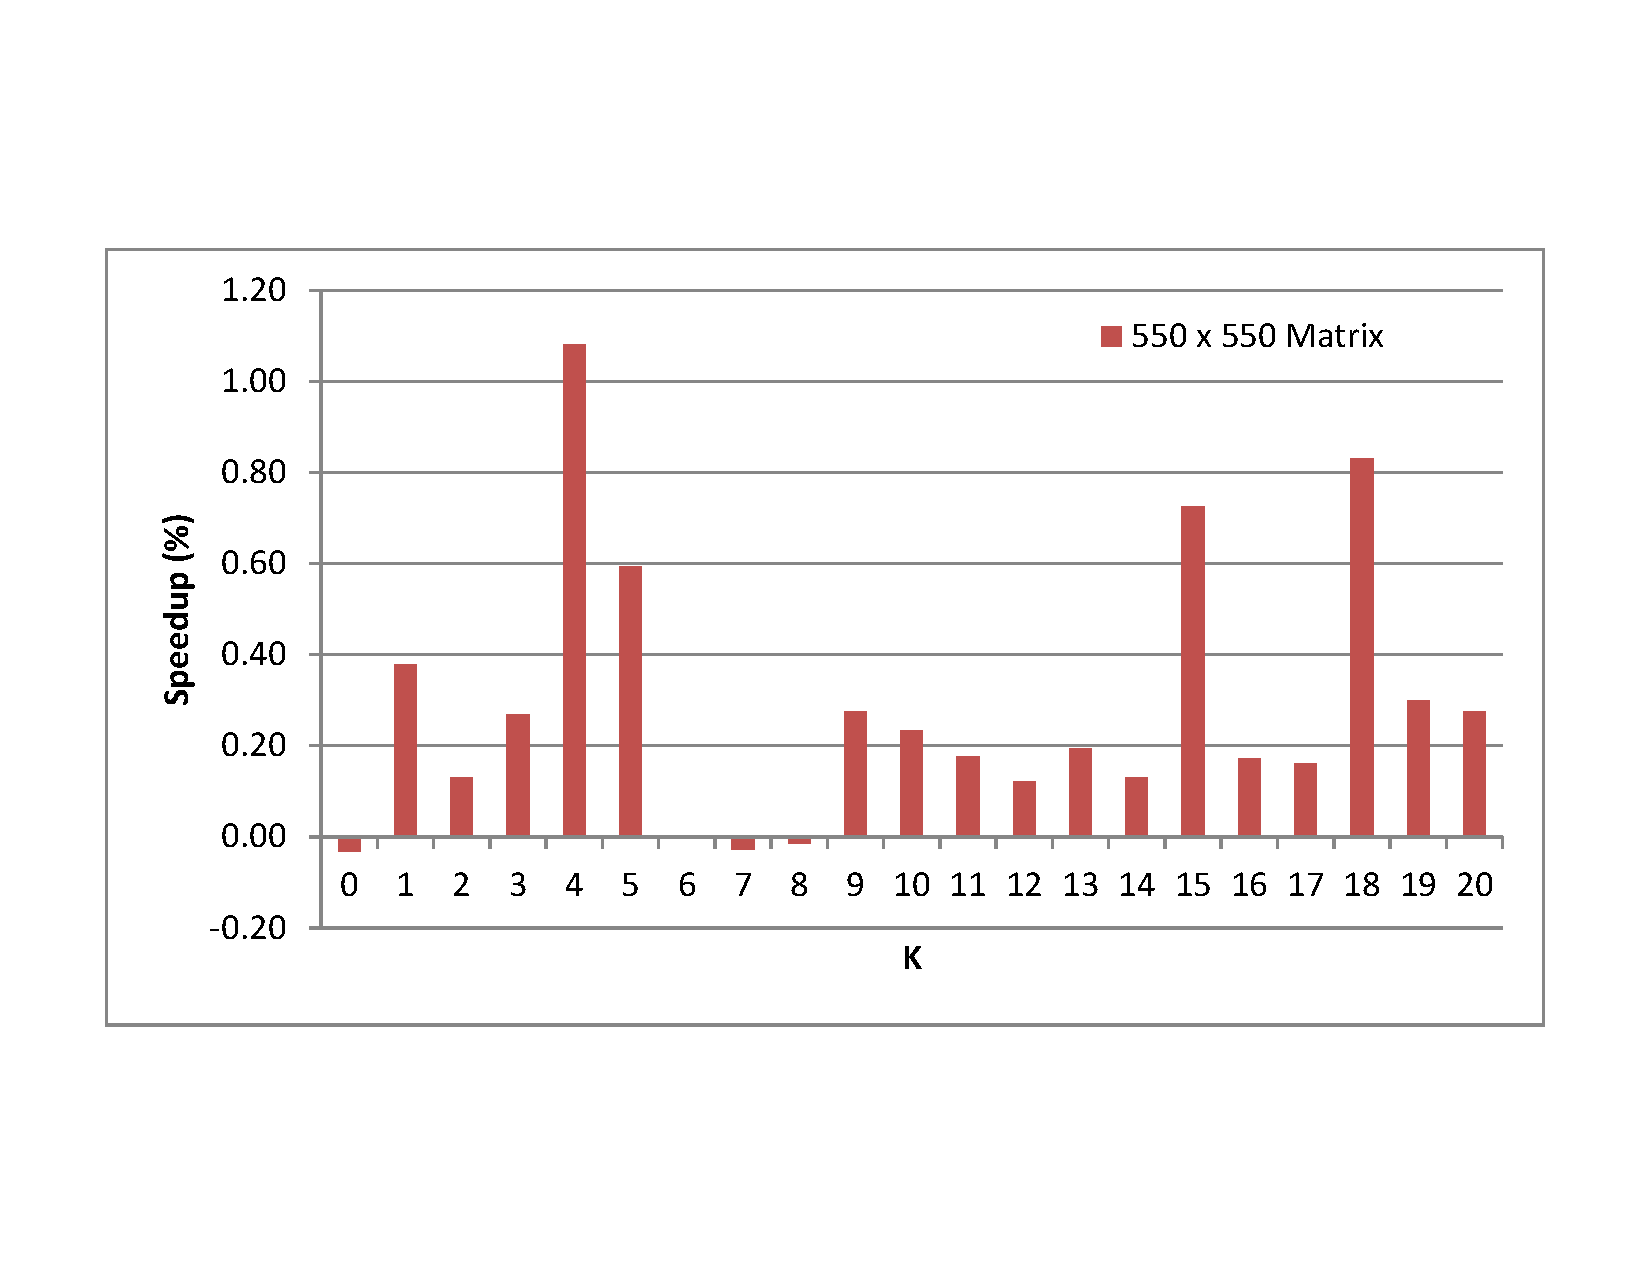
\includegraphics[scale=0.35]{./results/test_matrix3}
      \caption{Complex matrix multiplication with varying K\label{test_matrix3}}
    \end{minipage}
  \end{figure} 
  \begin{figure}[h]
    \begin{minipage} [t] {8.6cm}
      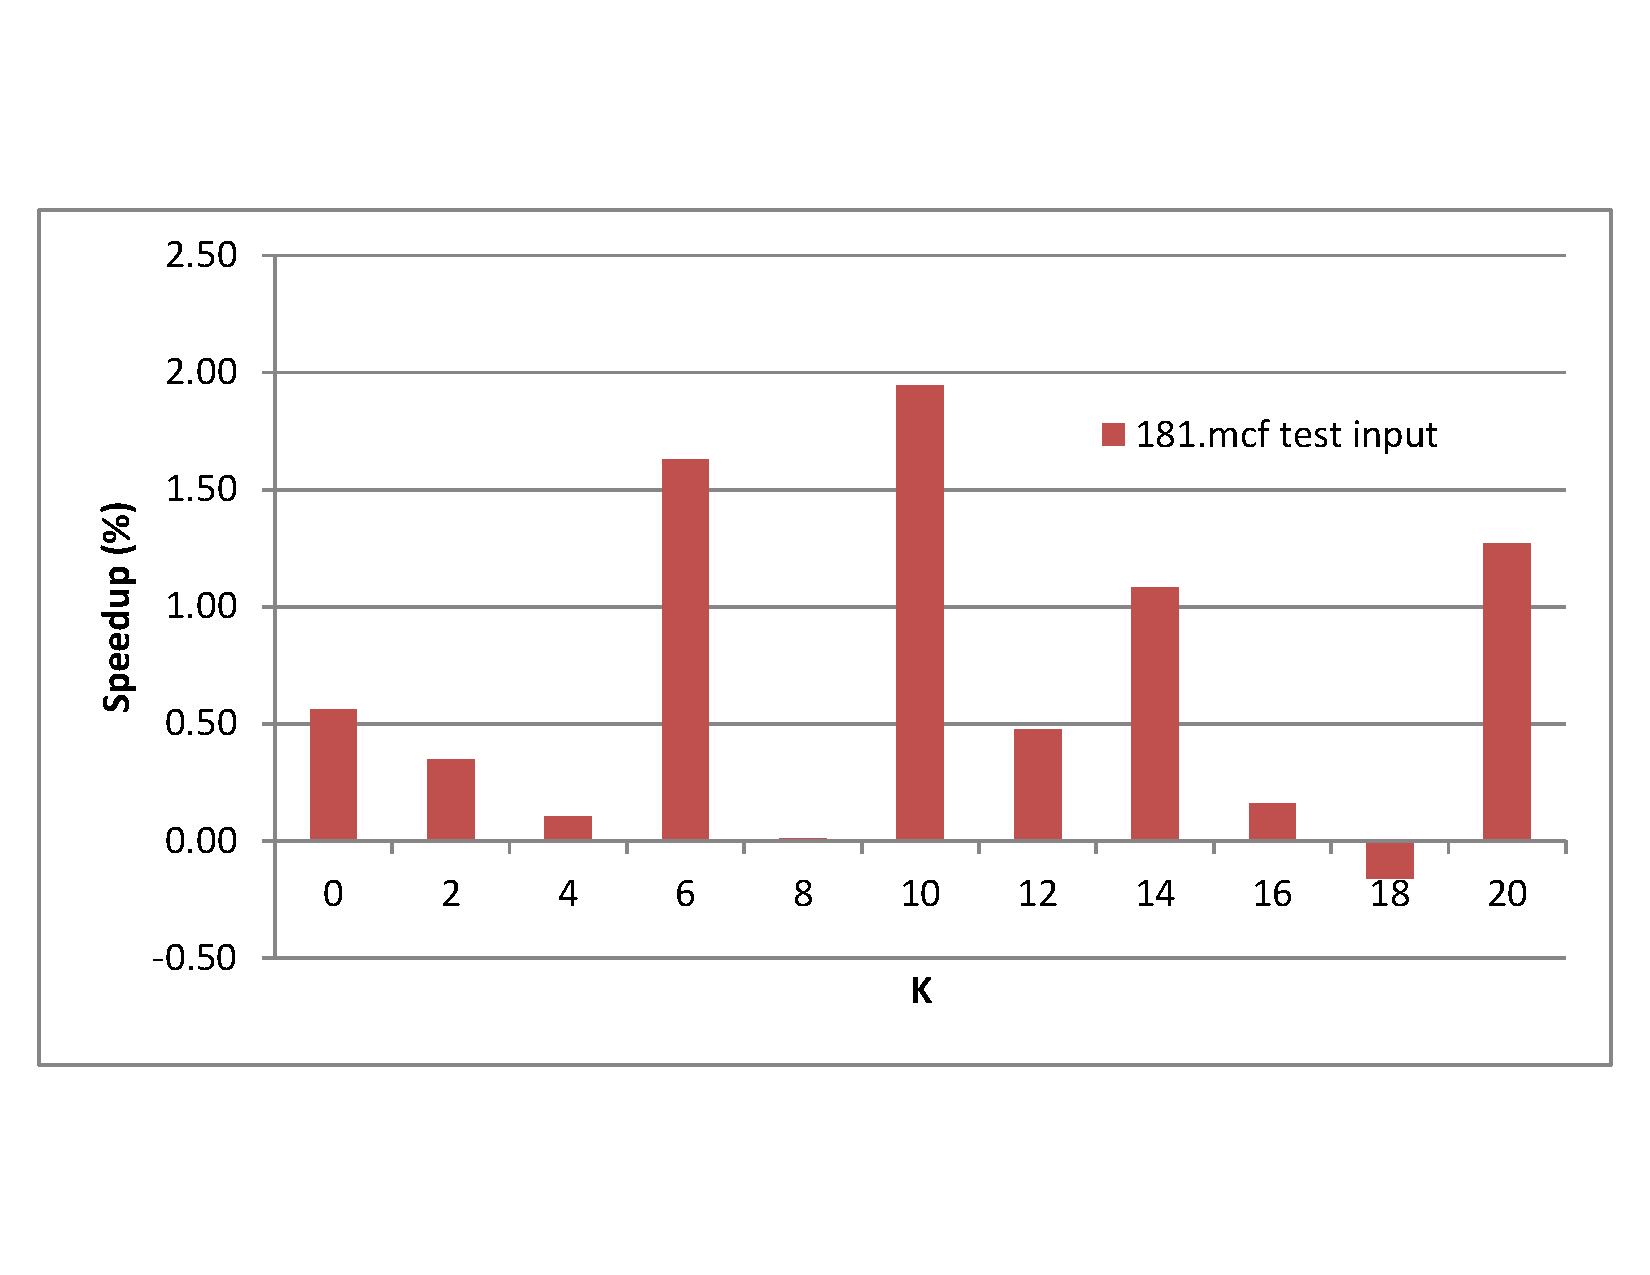
\includegraphics[scale=0.315]{./results/181_best_perf}
      \caption{SPECINT2000 181.mcf with varying K and test input\label{181}}
    \end{minipage}
    \begin{minipage} [t] {8.5cm}
      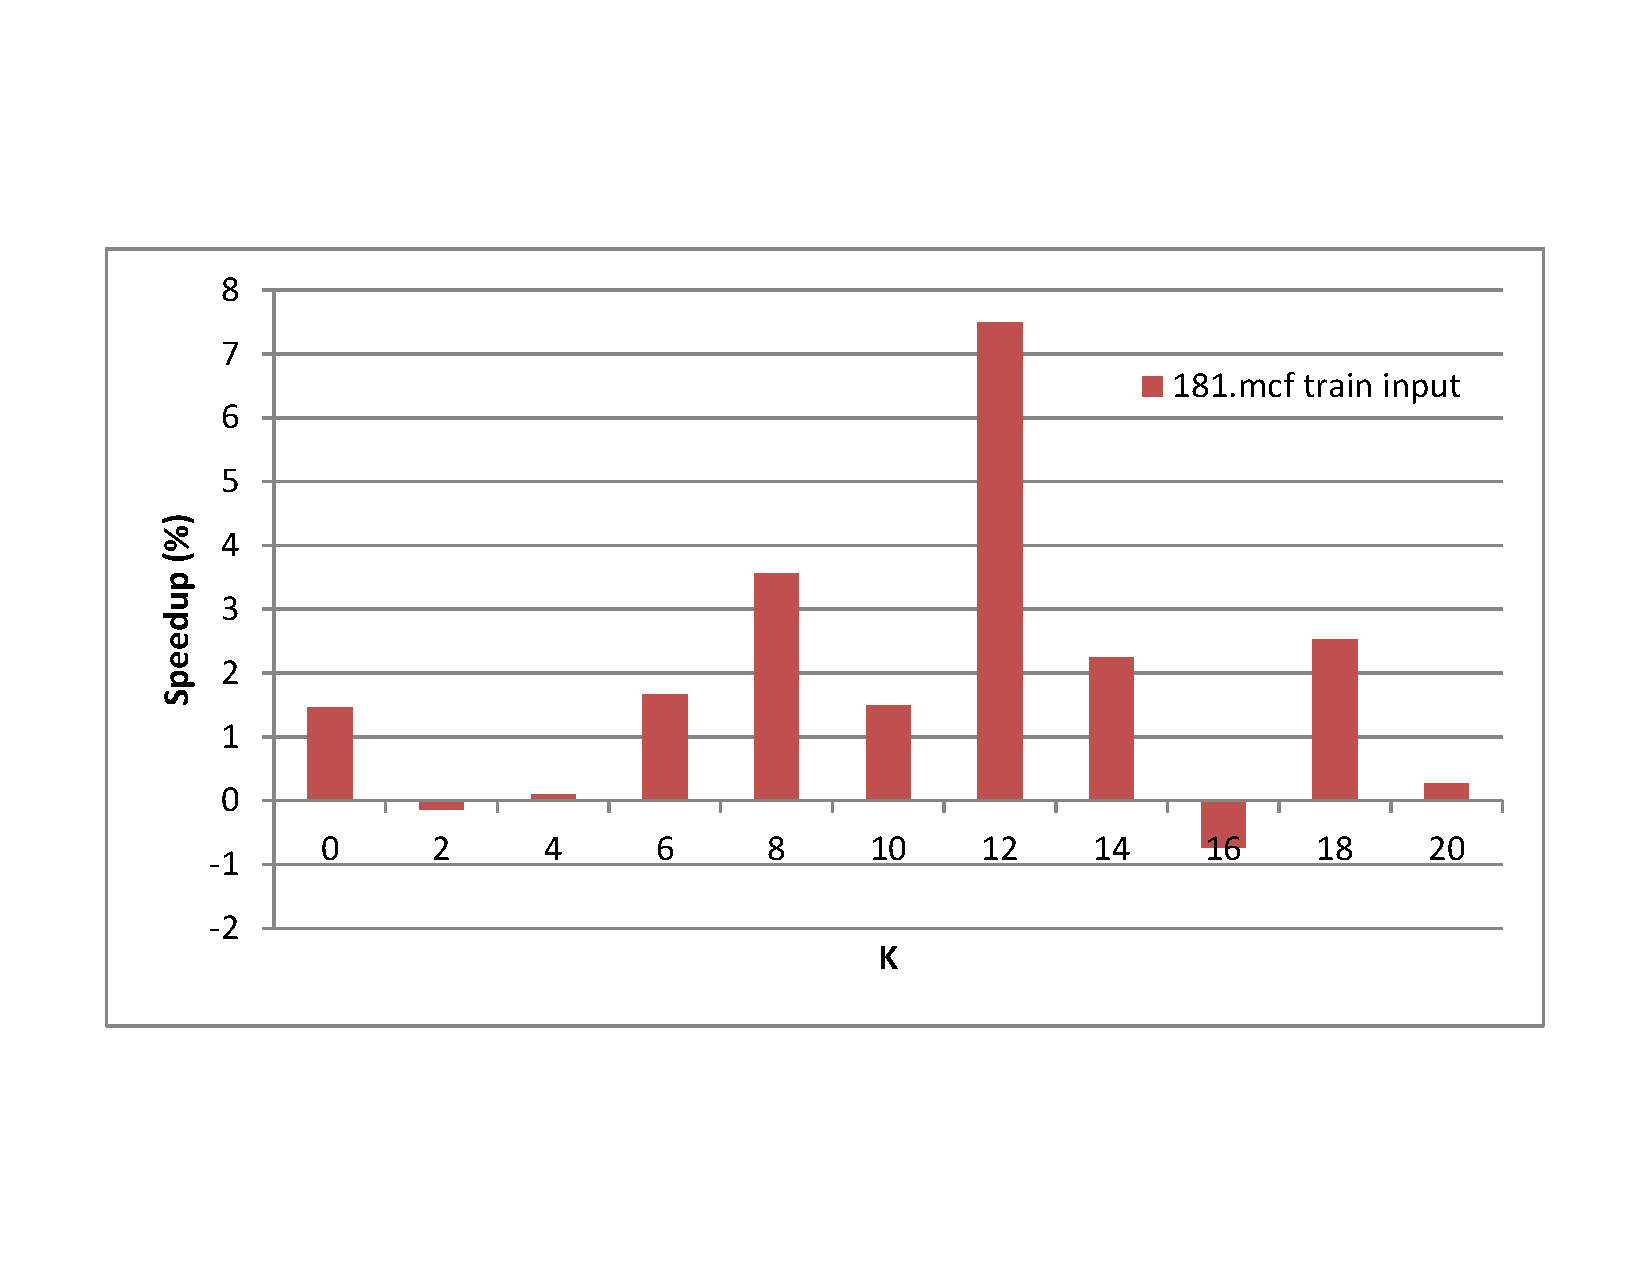
\includegraphics[scale=0.35]{./results/181train}
      \caption{SPECINT2000 181.mcf with varying K and train input\label{181}}
    \end{minipage}
  \end{figure} 

  tada citationg ~\cite{Wu2002} ~\cite{WuEtAl2002}
  ~\cite{metcalf93} ~\cite{prefetchsupportwebsite} ~\cite{dundas97} ~\cite{mowry98} ~\cite{luk99}
  \section{Conclusion}
  In our project, we guide the compiler to insert prefetching instructions for stride patterns. We followed the work of Youfeng Wu~\cite{Wu2002}. Our implementation of prefetching did show a speed up for our test cases thus confirming the work of~\cite{Wu2002}; our results showed speed up on the SPECINT benchmark test cases that we ran. We found that the profiling of these large programs required too much memory and time to run on our servers. Additionally, the efficiency of hardware prefetchers makes it hard to show improvement, and not slow down their cache schemes and we were not able to get detailed memory latency information~\cite{dahlgren95}. 
  \\\\With future work, we would get more detailed cache information and calculate a more efficient K using a hot trace inside of the loop. Presently, if the instruction count varies a lot based on control flow, our K value is inaccurate. A more accurate prefetch could be made with this information. The implementation for determing this sort of hot path to determing K would include counting number of cycles in the loop body which could be taken without taking the miss latency of the
  prefetched loads into account. Using the executiong count of the loop and whether a threshold was met for taking branches we could only concern ourselves with one path taken thus yielding a better estimate for AC [TODO REFERENCE THE EQUATION]. A more accurate AC gives us then a more accurate K and improve performance gained from prefetching.  

  \bibliography{paper}{}
  \bibliographystyle{plain}
  \end{document}
